\label{chapt:standards}

The driving parameter for this analysis is the drum's outer diameter (OD) $D$. For the entirety of this report, this value is constant at $D = 28\Unit{in} = 711\Unit{mm}$. Based on this fixed parameter, other relevant values used in this report are summarized below in Table~\ref{table:prelim_params}. All material properties selected as per John Umina's  suggestion from Table 1A of \cite{ASMEbvpcIID} for a SA-106 Grade B steel (most commonly used in seamless mechanical pipe). Units shown in both metric (SI) and United States customary (USC).\\

\begin{table}[ht]
	\caption{Key drum parameters and material properties.}
	\centering
	\begin{tabular}{lccccc}
		&       & \multicolumn{2}{c}{\textbf{\textit{SI}}} & \multicolumn{2}{c}{\textbf{\textit{UCS}}} \\
		\textbf{Description} & \textbf{Symbol} & \textbf{Value} & \textbf{Units} & \textbf{Value}  & \textbf{Units} \\
		\midrule
		Outer diameter       & $D$           & $711.2$        & $\Unit{mm}$           & $28$            & $\Unit{in}$           \\
		Tether diameter      & $d$       	   & $15.2$         & $\Unit{mm}$           & $0.598$         & $\Unit{in}$           \\
		Drum length          & $L$             & $1,244.6$      & $\Unit{mm}$           & $49$            & $\Unit{in}$           \\
		Tether tension       & $T$             & $51,264$       & $\Unit{N}$            & $11,525$        & $\Unit{lbf}$          \\
		Yield strength       & $\sigma_y$           & $241.3$        & $\Unit{MPa}$          & $35,000$        & $\Unit{psi}$          \\
		Young's modulus      & $E$             & $200$          & $\Unit{GPa}$          & $2.9\cdot 10^7$ & $\Unit{psi}$          \\
		Poisson's ratio      & $\nu$           & $0.3$          & $-$            		& $-$             & $-$           		  \\
		Safety factor        & $n$            & $1.5$          & $-$            		& $-$             & $-$            	      \\
	\end{tabular}%
	\label{table:prelim_params}
\end{table}

The best approach to this problem is to model the drum as an externally pressured vessel. First, in order to make this approximation, it is required to investigate how the tether tension is translated into a pressure. This will be done by reviewing the derivation for the Capstan Equation as per Ephraim Lanford's suggestion.\\ 

Next, using the above parameters and pressure, it was suggested by John Umina that the following codes and standards should be investigated for determining the required drum barrel thickness.
\begin{itemize}
	\item American Society of Mechanical Engineers (ASME):
	      \begin{itemize}[label=$\bullet$]
	      	\item Boiler and Pressure Vessel Code, Section VIII, Division 1 \cite{ASMEbvpcVII1}
	      	\item Boiler and Pressure Vessel Code, Section VIII, Division 2 \cite{ASMEbvpcVII2}
	      \end{itemize}
	\item European Standard EN
	      \begin{itemize}[label=$\bullet$]
	      	\item EN 13445: Unfired Pressure Vessels, Part 3: Design \cite{EN134453}
	      \end{itemize}
	\item Det Norske Veritas(DNV)
	      \begin{itemize}[label=$\bullet$]
	      	\item DNV-OS-D101, Marine and Machinery Systems and Equipment \cite{DNVOSD101}
	      \end{itemize}
	\item Thin Walled Pressure Vessel (TWPV) Hoop Stress \cite{roarks}\\	
\end{itemize}

Please note that all symbols used in the foregoing sections will follow those from their respective references, for clarity.
%----------------------------------------------------------------------------------------------------------------------
\section{Capstan Equation}
It is required to understand how one wrap of tether in tension causes an external pressure $p$ on the outer surface of the drum. The solution reveals itself in the derivation of the well-known Capstan relation or Equation~\ref{eq:Capstan} \cite{capstanman}.

\begin{equation}
	\label{eq:Capstan}
	T_2 = T_1 e^{\mu\theta}
\end{equation}

Where $T_1$ is the hold force and $T_2$ is the pull force (i.e. $T_2 \geq T_1$). This equation can also be rewritten as \ref{eq:Capstan_mod} for the instantaneous hold force as a function of contact angle, where $T_0$ is the applied tether tension. 

\begin{equation}
	\label{eq:Capstan_mod}
	T(\theta) = T_0 e^{-\mu\theta}
\end{equation}

From this equation, the free body diagram that leads to the above solutions is presented below in Figure~\ref{fig:Capstan}~\cite{capstanman}. 

\begin{figure}[H]
	\centering
	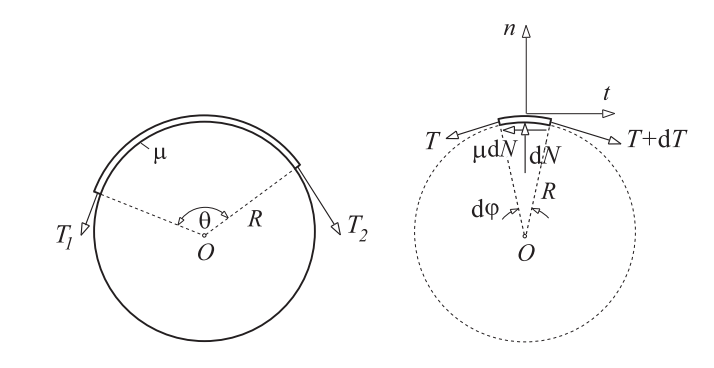
\includegraphics[scale=0.75]{2_Capstan}
	\caption[Free body diagram of differential capstan problem.]{Free body diagram of differential capstan problem. \protect\cite{capstanman}}
	\label{fig:Capstan}
\end{figure}

From above, it is clear that to extrapolate a pressure $p$ from the applied tension $T$, an equation for the equivalent normal force $N$ must be determined. This is done by performing a force balance in the normal direction $\hat{n}$ ($\Sigma F_{\hat{n}} = 0 $) which reduces to Equation~\ref{eq:CapstanSigRad}.

\begin{equation}
	\label{eq:CapstanSigRad}
	dN-(T+dT)\sin \frac{d\varphi}{2}+T\sin \frac{d\varphi}{2}= 0
\end{equation}

By assuming a small change in angle, the following substitutions are made: $\sin \varphi \approx \varphi$ and $dT d\varphi/2 \approx 0$. Applying these relations to \ref{eq:CapstanSigRad} leaves \ref{eq:diffNormal}.

\begin{equation}
	\label{eq:diffNormal}
	dN = T d\varphi
\end{equation}

The relation from Equation~\ref{eq:diffNormal} will be key for the following derivations. The overall normal force $N$ caused by the tether tension $T$ can be solved for by integration \ref{eq:capstan_integral} yielding \ref{eq:CapstanNorm}.

\begin{equation}
	\label{eq:capstan_integral}
	\int_0^N dN =\int_0^{2\pi} T d\varphi
\end{equation}

\begin{equation}
	\label{eq:CapstanNorm}
	N=2\pi T	
\end{equation}

With this resultant normal force over one revolution of tether, it is now apparent that the pressure $p$ can be solved for by distributing $N$ over this area as seen in Equation~\ref{eq:2_preq}.

\begin{equation}
	\label{eq:2_preq}
	p=\frac{N}{A}=\frac{2\pi T}{d\pi D}=\frac{2T}{Dd}
\end{equation}

Using the values from Table~\ref{table:prelim_params} and Equation~\ref{eq:2_preq}, $p=1376\Unit{psi}= 9.484\Unit{MPa}$. Note that Equation~\ref{eq:2_preq} is independent of the number of tether revolutions (i.e. both $N$ and $A$ scale by a factor of $2\pi n$ wraps). This behavior is next investigated.

%------------------------------------------------------------------------------------------
\subsection{Alternate Solution}
\label{subsection:alt}

An alternate solution can be found by substituting \ref{eq:Capstan_mod} in \ref{eq:capstan_integral}, becoming \ref{eq:capstan_integral2} and yielding \ref{eq:CapstanNorm2} (recall $\int e^{ax} dx = \tfrac{1}{a} e^{ax} + C$).

\begin{equation}
	\label{eq:capstan_integral2}
	\begin{aligned}
		\int_0^N dN =\int_0^{\theta} T_{0} e^{-\mu \varphi} d\varphi            \\
		N = \left( -\frac{T_{0}}{\mu} e^{-\mu \varphi} \right) \Big|_0^{\theta} 
	\end{aligned}
\end{equation}

\begin{equation}
	\label{eq:CapstanNorm2}
	N = \frac{T_{0}}{\mu} \left( 1 - e^{-\mu \theta} \right)
\end{equation}

This equation represents the stored normal force given a contact angle $\theta$. To find $p$ as a function $\theta$, $N$ is distributed over the cumulative area as seen in Equation~\ref{eq:2_preq2}.

\begin{equation}
	\label{eq:2_preq2}
	p=\frac{N}{A}= \frac{T_{0} \left( 1 - e^{-\mu \theta} \right)}{\mu d R \theta}
\end{equation}

Using a Python script \cite{PYTHON} from Appendix~\ref{appendix:a0}, the following plots in Figures~\ref{fig:2_nvar} and \ref{fig:2_pvar} below show the variation in normal force $N$ and pressure $p$ for coefficient of friction values $\mu \in [0.05, 0.50]$.

\begin{figure}[H]
	\centering
	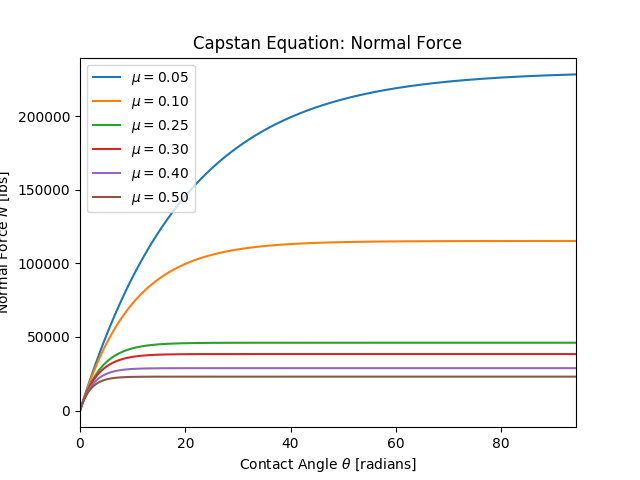
\includegraphics[scale=0.75]{2_nvar}
	\caption{Variation of stored normal force $N$ versus contact angle $\theta$.}
	\label{fig:2_nvar}
\end{figure}

\begin{figure}[H]
	\centering
	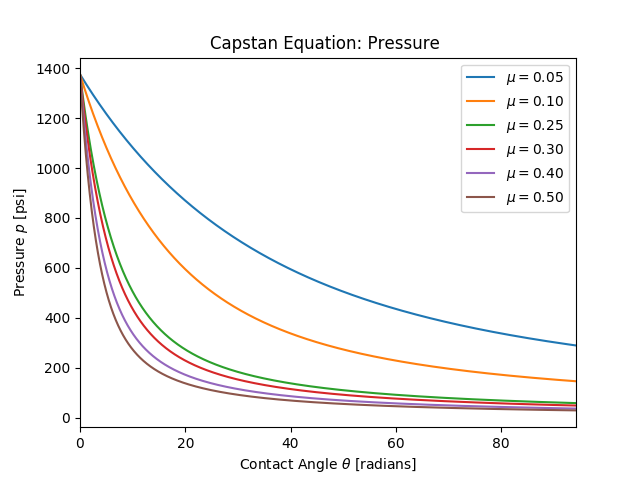
\includegraphics[scale=0.75]{2_pvar}
	\caption{Variation of pressure $p$ versus contact angle $\theta$.}
	\label{fig:2_pvar}
\end{figure}

Several observations may be made from these plots. For instance, as the contact angle increases, the stored normal force has an asymptomatic behavior. This behavior coupled with the increase in area results in a pressure which goes to zero after several wraps $n$ (i.e. $2 \pi n \Unit{Radians}$). Furthermore, as the coefficient of friction between the tether and the drum increases, the decay in pressure is quicker. A key observation to be made is that regardless of the $\mu$, all initial pressures $p(0)$ start at the value calculated from Equation~\ref{eq:2_preq}.  

%%----------------------------------------------------------------------------------------------------------------------
\section{ASME's BPVC}

The ASME Boiler and Pressure Vessel Codes (BPVC) listed at the beginning of this chapter are next extensively studied. Note that for all iteration procedures in the following subsections, an initial thickness of $t_0 =0.500\Unit{in}= 12.7 \Unit{mm}$ with a step of  $0.01\Unit{in} \ / \ 0.254\Unit{mm}$ is used. Python scripts \cite{PYTHON} utilized for implementing the solving algorithms are found in Appendix~A. 
\subsection{Section VIII: Division 1}
\label{section:2_VIII1}
As per subsection UG-28 of \cite{ASMEbvpcVII1}, the following procedure is used to calculate the required thickness.

\begin{enumerate}
	\item Assume initial thickness value of $t_0$
	\item Calculate $D/t$ ratio and assure $D/t \geq 10$.
	\item Calculate $L/D$ ratio, if $L/D \geq 50 \Rightarrow 50$ or  $L/D \leq 0.05 \Rightarrow 0.05$
	\item With the above ratios, go to Figure G of \cite{ASMEbvpcIID} and get value for $A$
	\item With $A$ from above go to chart CS-2 $\because \sigma_y \geq 30,000 \Unit{psi}$ to get $B$
	\item Use Equation \ref{eq:2_VII1_pa} with $B$ to calculate allowable pressure $p_a$:
	      \begin{equation}
	      	\label{eq:2_VII1_pa}
	      	p_a = \frac{4B}{3 \left(D/t\right)}
	      \end{equation}
	\item Check that $p_a \geq p_{req}$ as calculated from Equation~\ref{eq:2_preq}, if not, increase $t$, go to Step 2 and repeat\\
	      	
\end{enumerate}

Convergence is plotted with the script from Appendix~\ref{appendix:a1} (see Figure~\ref{fig:2_vii1_cnvg}).
\begin{figure}[H]
	\centering
	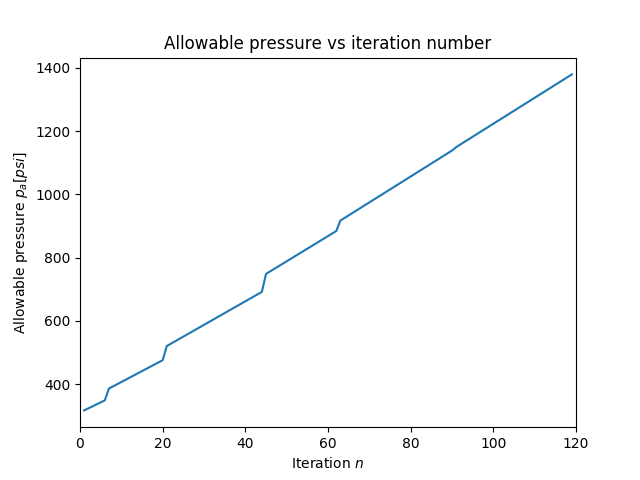
\includegraphics[scale=0.75]{2_vii1_cnvg}
	\caption{Convergence plot of $p_a$ using ASME's BPVC VIII-1.}
	\label{fig:2_vii1_cnvg}
\end{figure}

From this plot, the script converged at thickness of $t = 1.680\Unit{in} = 43.7\Unit{mm}$ when $p_a\geq p_{req}$ after $n=119$ iterations. 


\subsection{Section VIII: Division 2}
\label{section:2_VIII2}
As per subsection 4.4.5 of \cite{ASMEbvpcVII2}, the following procedure is used to calculate the required thickness. Note that only the main formulas will be presented. For intermediate steps, see  the Python script in Appendix~\ref{appendix:a2}.
\begin{enumerate}
	\item Assume initial thickness value of $t_0$
	\item Calculate elastic buckling stress $F_{he}$ with Equation~\ref{eq:2_VII2_4419}
	      \begin{equation}
	      	\label{eq:2_VII2_4419}
	      	F_{he} = \frac{1.6\ C_h E_y t}{D}
	      \end{equation}
	\item Based on $\sigma_y$ and $F_{he}$, calculate the predicted buckling stress $F_{ic}$
	\item With subsection 4.4.2 of \cite{ASMEbvpcVII2}, compute the design factor $FS$
	\item Calculate allowable pressure $p_a$ with Equation~\ref{eq:2_VII2_4428}
	      \begin{equation}
	      	\label{eq:2_VII2_4428}
	      	p_a = 2 F_{ha} \left(\frac{t}{D}\right)
	      \end{equation}
	\item Check if $p_a \geq p_{req}$ as calculated from \ref{eq:2_preq}, if not, increase $t$, return to Step 2 and repeat \\
	      	
\end{enumerate}

%%on page~\pageref{fig:2_vii2_cnvg} for page ref
The script in Appendix~\ref{appendix:a2} plots convergence as seen in Figure~\ref{fig:2_vii2_cnvg}.
\begin{figure}[H]
	\centering
	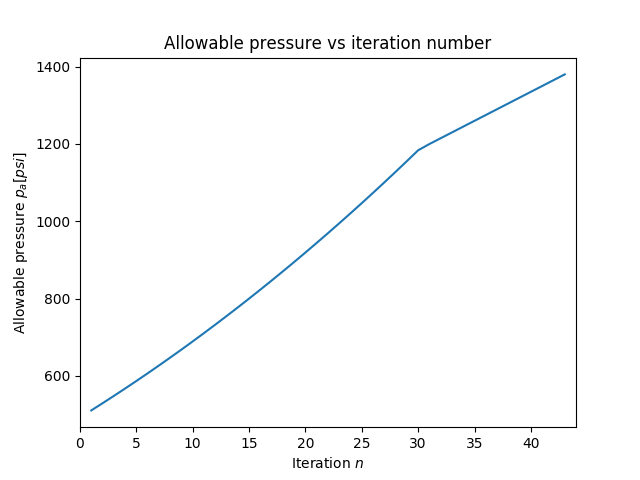
\includegraphics[scale=0.75]{2_vii2_cnvg}
	\caption{Convergence plot of $p_a$ using ASME's BPVC VIII-2.}
	\label{fig:2_vii2_cnvg}
\end{figure}

Convergence is reached at a thickness of $t = 0.920\Unit{in}= 23.4\Unit{mm}$ when $p_a\geq p_{req}$, after $n=43$ iterations. 


%%----------------------------------------------------------------------------------------------------------------------
\section{European Standard}
\subsection{EN-13445-3}
\label{section:2_EN}
As per subsection 8.5.2.2 of \cite{EN134453}, the following procedure is used to calculate the required thickness $e_a$. Note that the script in Appendix~\ref{appendix:a3} utilizes SI units as per \cite{EN134453}.

\begin{enumerate}
	\item Assume initial thickness value of $e_a$ and calculate $p_y$ with \ref{eq:2_EN_py}
	      \begin{equation}
	      	\label{eq:2_EN_py}
	      	p_y = \frac{\sigma_e e_a}{R}
	      \end{equation}
	\item Compute the lower failure pressure $p_m$ \ref{eq:2_EN_pm}, see 8.5.2.6 of \cite{EN134453} for $\varepsilon$
	      \begin{equation}
	      	\label{eq:2_EN_pm}
	      	p_m = \frac{E e_a  \varepsilon}{R}
	      \end{equation}
	\item With the $p_m/p_y$ ratio, use Figure 8.5.5 of \cite{EN134453} to find equivalent $p_r/p_y$
	\item Rearrange for $p_r$ and calculate allowable pressure $p$ ith \ref{eq:2_EN_pa}
	      \begin{equation}
	      	\label{eq:2_EN_pa}
	      	p = \frac{p_r}{S}
	      \end{equation}
	\item Check if $p \geq p_{req}$ as calculated from \ref{eq:2_preq} otherwise, increase $e_a$, return to Step 2 and repeat\\
\end{enumerate}

Again, with the script from Appendix~\ref{appendix:a3}, convergence is shown(see Figure~\ref{fig:2_en13445_cnvg}).
\begin{figure}[H]
	\centering
	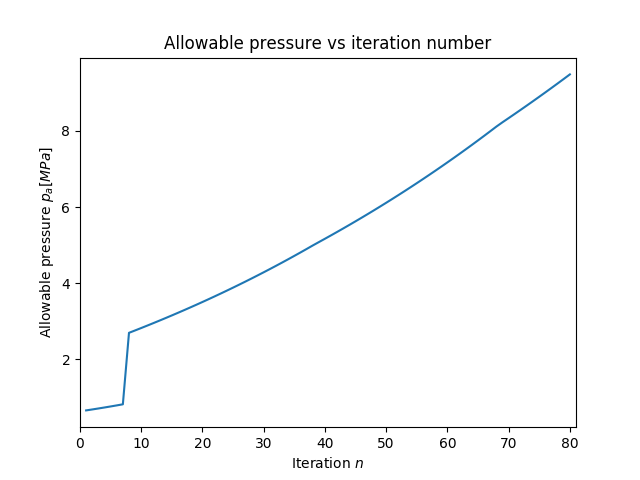
\includegraphics[scale=0.75]{2_en13445_cnvg}
	\caption{Convergence plot of $p_a$ using EN 13445-3.}
	\label{fig:2_en13445_cnvg}
\end{figure}

The script converged at thickness of $e_a = 32.8\Unit{mm} = 1.290\Unit{in}$ and an allowable pressure of $p\geq p_{req}$ after $n=80$ iterations. 

%%----------------------------------------------------------------------------------------------------------------------
\section{DNV}

\subsection{DNV-OS-D101}
\label{section:2_DNV}

As per \cite{DNVOSD101}, in subsection F215, Equation~\ref{eq:2_DNV_hoop} is presented as follows.

\begin{equation}
	\label{eq:2_DNV_hoop}
	\sigma_h = C\cdot\frac{T}{d_{thr}t}
\end{equation}

In this equation, $C$ is a factor based on the number of wraps on the drum. For this application with two layers, $C=1.75$ \cite{DNVOSD101}. There are a few exceptions with this equation and they are listed as follows.

\begin{enumerate}
	\item The hoop stress $\sigma_h$ is limited to $\sigma_h \leq 0.85\cdot \sigma_y$
	\item The calculated $\sigma_h$  may only be superseded with larger tested value\\
\end{enumerate}

For the remainder of this report, the allowable stress limit $\sigma_a$ will be presented as Equation~\ref{eq:2_sigall}.

\begin{equation}
	\label{eq:2_sigall}
	\sigma_a = \frac{\sigma_y}{n}
\end{equation}

By substituting yield strength and safety factor values from Table~\ref{table:prelim_params}, $\therefore \sigma_a= 23,333 \Unit{psi}= 160.9 \Unit{MPa}$.\\

Rearranging Equation~\ref{eq:2_DNV_hoop} for $t$ and setting $\sigma_h$ to the above calculated limit, solving accordingly will yield a valid value of $t = 1.440 \Unit{in} = 36.6\Unit{mm}$. 

%----------------------------------------------------------------------------------------------------------------------
\section{TWPV Hoop Stress}
\label{section:2_TWPV}

A final preliminary benchmarking step studies the hoop stress equation \cite{roarks} for a TWPV. From this, Equation~\ref{eq:2_hoop} is presented as follows.

\begin{equation}
	\label{eq:2_hoop}
	\sigma_h = \frac{pR}{t}
\end{equation}

Again, rearranging for $t$ , $\sigma_h=\sigma_a$ and using the pressure $p$ calculated from Equation~\ref{eq:2_preq}, a value of $t =0.825 \Unit{in}=21.0\Unit{mm}$ is calculated. Note that $\because R/t = 17 \geq 10$, the assumption of a TWPV is valid.

%%----------------------------------------------------------------------------------------------------------------------
\section{Comparison}

Based on the results determined in this section, a summary is presented in Table~\ref{table:2_comp} below.
\begin{table}[H]
	\centering
	\caption{Comparison of calculated $t$ with corresponding method.}
	\begin{tabular}{lccc}
		\textbf{Method}  & \textbf{$mm$} & \textbf{$in$} & \textbf{$n$} \\
		\midrule
		ASME BPVC VIII-1 & $43.7$                 & $1.680$                & $1.5$       \\
		ASME BPVC VIII-2 & $23.4$                 & $0.920$                & $1.5$       \\
		EN 13445-3       & $32.8$                 & $1.290$                & $1.5$       \\    
		DNV-OS-D101      & $36.6$                 & $1.440$                & $1.5$       \\
		TWPV Hoop Stress & $21.0$                 & $0.825$                & $1.5$       \\
	\end{tabular}%
	\label{table:2_comp}%
\end{table}%

The following observations are made from this tabular summary:
\begin{itemize}
	\item ASME's BPVC VIII-1 yields the most conservative $t$
	\item TWPV Hoop Stress \& ASME's BPVC VIII-2 yield both low $t$ values 
	\item EN 13445-3 \& DNV-OS-D101 lie in between \\
\end{itemize}

The results from this section serve as an excellent benchmark for the range of expected values (i.e. $t\in[0.825,1.680]$ in). In the following section, an analytical approach will be taken in hopes of closing in on a drum barrel thickness.